\documentclass{standalone}
\usepackage{tikz}
\usetikzlibrary{patterns, positioning}

\begin{document}
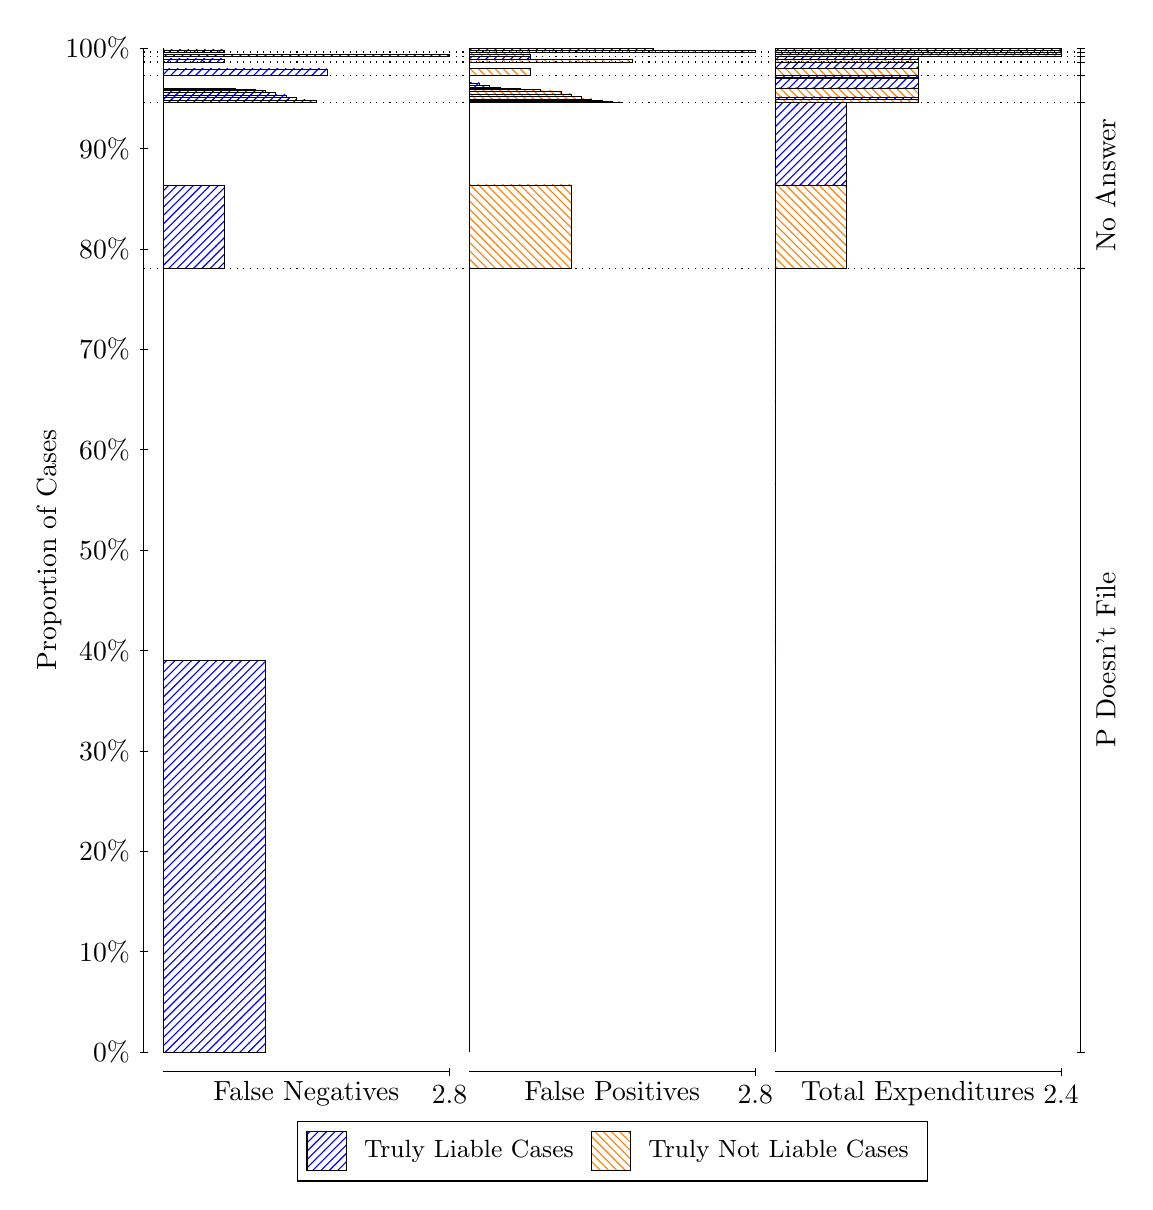
\begin{tikzpicture}
\draw[black, very thin] (1.5,1.75) -- (1.5,14.5);
\node[rotate=90, anchor=center] at (0.3, 8.125) {Proportion of Cases};
\draw[black, very thin] (1.45,1.75) -- (1.55,1.75);
\node[anchor=east] at (1.45, 1.75) {0\%};
\draw[black, very thin] (1.45,3.025) -- (1.55,3.025);
\node[anchor=east] at (1.45, 3.025) {10\%};
\draw[black, very thin] (1.45,4.3) -- (1.55,4.3);
\node[anchor=east] at (1.45, 4.3) {20\%};
\draw[black, very thin] (1.45,5.575) -- (1.55,5.575);
\node[anchor=east] at (1.45, 5.575) {30\%};
\draw[black, very thin] (1.45,6.85) -- (1.55,6.85);
\node[anchor=east] at (1.45, 6.85) {40\%};
\draw[black, very thin] (1.45,8.125) -- (1.55,8.125);
\node[anchor=east] at (1.45, 8.125) {50\%};
\draw[black, very thin] (1.45,9.4) -- (1.55,9.4);
\node[anchor=east] at (1.45, 9.4) {60\%};
\draw[black, very thin] (1.45,10.675) -- (1.55,10.675);
\node[anchor=east] at (1.45, 10.675) {70\%};
\draw[black, very thin] (1.45,11.95) -- (1.55,11.95);
\node[anchor=east] at (1.45, 11.95) {80\%};
\draw[black, very thin] (1.45,13.225) -- (1.55,13.225);
\node[anchor=east] at (1.45, 13.225) {90\%};
\draw[black, very thin] (1.45,14.5) -- (1.55,14.5);
\node[anchor=east] at (1.45, 14.5) {100\%};

\draw[black, very thin] (13.4,1.75) -- (13.4,14.5);
\draw[black, very thin] (13.35,1.75) -- (13.45,1.75);
\node[anchor=west] at (13.35, 1.75) {};
\draw[black, very thin] (13.35,11.705) -- (13.45,11.705);
\node[anchor=west] at (13.35, 11.705) {};
\draw[black, very thin] (13.35,13.811) -- (13.45,13.811);
\node[anchor=west] at (13.35, 13.811) {};
\draw[black, very thin] (13.35,14.151) -- (13.45,14.151);
\node[anchor=west] at (13.35, 14.151) {};
\draw[black, very thin] (13.35,14.323) -- (13.45,14.323);
\node[anchor=west] at (13.35, 14.323) {};
\draw[black, very thin] (13.35,14.398) -- (13.45,14.398);
\node[anchor=west] at (13.35, 14.398) {};
\draw[black, very thin] (13.35,14.449) -- (13.45,14.449);
\node[anchor=west] at (13.35, 14.449) {};
\draw[black, very thin] (13.35,14.5) -- (13.45,14.5);
\node[anchor=west] at (13.35, 14.5) {};

\draw[black, very thin, pattern color=blue, pattern=north east lines] (1.75,1.75) rectangle (3.0476,6.7277);
\draw[black, very thin, pattern color=orange, pattern=north west lines] (1.75,6.7277) rectangle (1.75,11.705);
\draw[black, very thin, pattern color=blue, pattern=north east lines] (1.75,11.705) rectangle (2.5286,12.755);
\draw[black, very thin, pattern color=orange, pattern=north west lines] (1.75,12.755) rectangle (1.75,13.811);
\draw[black, very thin, pattern color=blue, pattern=north east lines] (1.75,13.811) rectangle (3.6964,13.831);
\draw[black, very thin, pattern color=blue, pattern=north east lines] (1.75,13.831) rectangle (3.5667,13.84);
\draw[black, very thin, pattern color=blue, pattern=north east lines] (1.75,13.84) rectangle (3.4369,13.872);
\draw[black, very thin, pattern color=blue, pattern=north east lines] (1.75,13.872) rectangle (3.3071,13.905);
\draw[black, very thin, pattern color=blue, pattern=north east lines] (1.75,13.905) rectangle (3.1774,13.941);
\draw[black, very thin, pattern color=blue, pattern=north east lines] (1.75,13.941) rectangle (3.0476,13.959);
\draw[black, very thin, pattern color=blue, pattern=north east lines] (1.75,13.959) rectangle (2.9179,13.973);
\draw[black, very thin, pattern color=blue, pattern=north east lines] (1.75,13.973) rectangle (2.7881,13.979);
\draw[black, very thin, pattern color=blue, pattern=north east lines] (1.75,13.979) rectangle (2.6583,13.985);
\draw[black, very thin, pattern color=orange, pattern=north west lines] (1.75,13.985) rectangle (1.75,14.151);
\draw[black, very thin, pattern color=blue, pattern=north east lines] (1.75,14.151) rectangle (3.8262,14.236);
\draw[black, very thin, pattern color=orange, pattern=north west lines] (1.75,14.236) rectangle (1.75,14.323);
\draw[black, very thin, pattern color=blue, pattern=north east lines] (1.75,14.323) rectangle (2.5286,14.362);
\draw[black, very thin, pattern color=orange, pattern=north west lines] (1.75,14.362) rectangle (1.75,14.398);
\draw[black, very thin, pattern color=blue, pattern=north east lines] (1.75,14.398) rectangle (5.3833,14.421);
\draw[black, very thin, pattern color=orange, pattern=north west lines] (1.75,14.421) rectangle (1.75,14.449);
\draw[black, very thin, pattern color=blue, pattern=north east lines] (1.75,14.449) rectangle (2.5286,14.476);
\draw[black, very thin, pattern color=orange, pattern=north west lines] (1.75,14.476) rectangle (1.75,14.5);
\draw[black, very thin, pattern color=orange, pattern=north west lines] (5.6333,1.75) rectangle (5.6333,6.7278);
\draw[black, very thin, pattern color=blue, pattern=north east lines] (5.6333,6.7278) rectangle (5.6333,11.705);
\draw[black, very thin, pattern color=orange, pattern=north west lines] (5.6333,11.705) rectangle (6.931,12.761);
\draw[black, very thin, pattern color=blue, pattern=north east lines] (5.6333,12.761) rectangle (5.6333,13.811);
\draw[black, very thin, pattern color=orange, pattern=north west lines] (5.6333,13.811) rectangle (7.5798,13.817);
\draw[black, very thin, pattern color=orange, pattern=north west lines] (5.6333,13.817) rectangle (7.45,13.823);
\draw[black, very thin, pattern color=orange, pattern=north west lines] (5.6333,13.823) rectangle (7.3202,13.835);
\draw[black, very thin, pattern color=orange, pattern=north west lines] (5.6333,13.835) rectangle (7.1905,13.853);
\draw[black, very thin, pattern color=orange, pattern=north west lines] (5.6333,13.853) rectangle (7.0607,13.886);
\draw[black, very thin, pattern color=orange, pattern=north west lines] (5.6333,13.886) rectangle (6.931,13.917);
\draw[black, very thin, pattern color=orange, pattern=north west lines] (5.6333,13.917) rectangle (6.8012,13.947);
\draw[black, very thin, pattern color=orange, pattern=north west lines] (5.6333,13.947) rectangle (6.6714,13.956);
\draw[black, very thin, pattern color=orange, pattern=north west lines] (5.6333,13.956) rectangle (6.5417,13.977);
\draw[black, very thin, pattern color=blue, pattern=north east lines] (5.6333,13.977) rectangle (6.2821,13.983);
\draw[black, very thin, pattern color=blue, pattern=north east lines] (5.6333,13.983) rectangle (6.1524,13.989);
\draw[black, very thin, pattern color=blue, pattern=north east lines] (5.6333,13.989) rectangle (6.0226,14.003);
\draw[black, very thin, pattern color=blue, pattern=north east lines] (5.6333,14.003) rectangle (5.8929,14.021);
\draw[black, very thin, pattern color=blue, pattern=north east lines] (5.6333,14.021) rectangle (5.7631,14.057);
\draw[black, very thin, pattern color=blue, pattern=north east lines] (5.6333,14.057) rectangle (5.6333,14.151);
\draw[black, very thin, pattern color=orange, pattern=north west lines] (5.6333,14.151) rectangle (6.4119,14.239);
\draw[black, very thin, pattern color=blue, pattern=north east lines] (5.6333,14.239) rectangle (5.6333,14.323);
\draw[black, very thin, pattern color=orange, pattern=north west lines] (5.6333,14.323) rectangle (7.7095,14.359);
\draw[black, very thin, pattern color=blue, pattern=north east lines] (5.6333,14.359) rectangle (6.4119,14.398);
\draw[black, very thin, pattern color=orange, pattern=north west lines] (5.6333,14.398) rectangle (6.4119,14.426);
\draw[black, very thin, pattern color=blue, pattern=north east lines] (5.6333,14.426) rectangle (5.6333,14.449);
\draw[black, very thin, pattern color=orange, pattern=north west lines] (5.6333,14.449) rectangle (9.2667,14.473);
\draw[black, very thin, pattern color=blue, pattern=north east lines] (5.6333,14.473) rectangle (7.969,14.5);
\draw[black, very thin, pattern color=orange, pattern=north west lines] (9.5167,1.75) rectangle (9.5167,6.7278);
\draw[black, very thin, pattern color=blue, pattern=north east lines] (9.5167,6.7278) rectangle (9.5167,11.705);
\draw[black, very thin, pattern color=orange, pattern=north west lines] (9.5167,11.705) rectangle (10.425,12.761);
\draw[black, very thin, pattern color=blue, pattern=north east lines] (9.5167,12.761) rectangle (10.425,13.811);
\draw[black, very thin, pattern color=orange, pattern=north west lines] (9.5167,13.811) rectangle (11.333,13.844);
\draw[black, very thin, pattern color=blue, pattern=north east lines] (9.5167,13.844) rectangle (11.333,13.88);
\draw[black, very thin, pattern color=orange, pattern=north west lines] (9.5167,13.88) rectangle (11.333,13.994);
\draw[black, very thin, pattern color=blue, pattern=north east lines] (9.5167,13.994) rectangle (11.333,14.113);
\draw[black, very thin, pattern color=orange, pattern=north west lines] (9.5167,14.113) rectangle (11.333,14.132);
\draw[black, very thin, pattern color=blue, pattern=north east lines] (9.5167,14.132) rectangle (11.333,14.151);
\draw[black, very thin, pattern color=orange, pattern=north west lines] (9.5167,14.151) rectangle (11.333,14.239);
\draw[black, very thin, pattern color=blue, pattern=north east lines] (9.5167,14.239) rectangle (11.333,14.323);
\draw[black, very thin, pattern color=orange, pattern=north west lines] (9.5167,14.323) rectangle (11.333,14.359);
\draw[black, very thin, pattern color=blue, pattern=north east lines] (9.5167,14.359) rectangle (11.333,14.398);
\draw[black, very thin, pattern color=orange, pattern=north west lines] (9.5167,14.398) rectangle (13.15,14.426);
\draw[black, very thin, pattern color=blue, pattern=north east lines] (9.5167,14.426) rectangle (13.15,14.449);
\draw[black, very thin, pattern color=orange, pattern=north west lines] (9.5167,14.449) rectangle (13.15,14.473);
\draw[black, very thin, pattern color=blue, pattern=north east lines] (9.5167,14.473) rectangle (13.15,14.5);
\draw[black, dotted] (1.5,11.705) -- (13.4,11.705);
\draw[black, dotted] (1.5,13.811) -- (13.4,13.811);
\draw[black, dotted] (1.5,14.151) -- (13.4,14.151);
\draw[black, dotted] (1.5,14.323) -- (13.4,14.323);
\draw[black, dotted] (1.5,14.398) -- (13.4,14.398);
\draw[black, dotted] (1.5,14.449) -- (13.4,14.449);
\draw[black, very thin] (1.75,1.5) -- (5.3833,1.5);
\node[anchor=north] at (3.5667, 1.5) {False Negatives};
\draw[black, very thin] (5.3833,1.45) -- (5.3833,1.55);
\node[anchor=north] at (5.3833, 1.45) {2.8};

\draw[black, very thin] (5.6333,1.5) -- (9.2667,1.5);
\node[anchor=north] at (7.45, 1.5) {False Positives};
\draw[black, very thin] (9.2667,1.45) -- (9.2667,1.55);
\node[anchor=north] at (9.2667, 1.45) {2.8};

\draw[black, very thin] (9.5167,1.5) -- (13.15,1.5);
\node[anchor=north] at (11.333, 1.5) {Total Expenditures};
\draw[black, very thin] (13.15,1.45) -- (13.15,1.55);
\node[anchor=north] at (13.15, 1.45) {2.4};

\node[black, centered, rotate=90] at (13.72, 6.7277) {P Doesn't File};
\node[black, centered, rotate=90] at (13.72, 12.758) {No Answer};






\draw (7.449999999999999,1.5) node[draw=none] (baseCoordinate) {};
\begin{scope}[align=center]
        \matrix[scale=0.5, draw=black, below=0.5cm of baseCoordinate, nodes={draw}, column sep=0.1cm]{
            \node[rectangle, draw, minimum width=0.5cm, minimum height=0.5cm, pattern=north east lines, pattern color=blue] {}; &
            \node[draw=none, font=\small] (B) {Truly Liable Cases}; &
            \node[rectangle, draw, minimum width=0.5cm, minimum height=0.5cm, pattern=north west lines, pattern color=orange] {}; &
            \node[draw=none, font=\small] (B) {Truly Not Liable Cases}; \\
            };
\end{scope}

\end{tikzpicture}
\end{document}